%% fig_cyclicmerge.tex   (generated by make_round42.py; do not edit by hand)
%% Collision of two branch points, two copies of SL(Y), and the induction on n (prop:cyclicmonodromy).
\documentclass[tikz,border=8pt]{standalone}
\usepackage{amsmath,amssymb}
\usetikzlibrary{arrows.meta,calc,decorations.pathreplacing}
%% palette.tex -- shared colour definitions for the figures
\definecolor{PInk}{RGB}{26,32,44}
\definecolor{PBlue}{RGB}{37,82,139}
\definecolor{PTeal}{RGB}{23,127,125}
\definecolor{POchre}{RGB}{193,138,44}
\definecolor{PClay}{RGB}{178,74,58}
\definecolor{PSlate}{RGB}{108,122,137}
\definecolor{PViolet}{RGB}{110,86,150}
\definecolor{WBlue}{RGB}{223,234,246}
\definecolor{WTeal}{RGB}{220,238,236}
\definecolor{WOchre}{RGB}{250,240,218}
\definecolor{WClay}{RGB}{247,229,224}
\definecolor{WSlate}{RGB}{238,241,244}
\definecolor{PMag}{RGB}{158,58,110}
\definecolor{PGrass}{RGB}{62,124,66}
\definecolor{PAmber}{RGB}{214,112,38}
\definecolor{PIndigo}{RGB}{58,64,140}
\definecolor{PRule}{RGB}{176,186,197}

%% shared macros so the standalone figures match the paper
\providecommand{\QQ}{\mathbb{Q}}
\providecommand{\ZZ}{\mathbb{Z}}
\providecommand{\RR}{\mathbb{R}}
\providecommand{\CC}{\mathbb{C}}
\providecommand{\PP}{\mathbb{P}}
\providecommand{\Kx}{K^{\times}}
\providecommand{\HW}{W}
\providecommand{\Nm}{\mathrm{N}}
\providecommand{\Hdg}{\mathrm{Hdg}}
\providecommand{\NS}{\mathrm{NS}}
\providecommand{\cA}{\mathcal{A}}
\providecommand{\cD}{\mathcal{D}}
\providecommand{\cF}{\mathcal{F}}
\providecommand{\cP}{\mathcal{P}}
\providecommand{\cO}{\mathcal{O}}
\providecommand{\cQ}{\mathcal{Q}}
\providecommand{\bbar}[1]{\overline{#1}}
\providecommand{\ch}{\operatorname{ch}}
\providecommand{\End}{\mathrm{End}}
\providecommand{\Ext}{\operatorname{Ext}}
\providecommand{\Supp}{\operatorname{Supp}}

\begin{document}
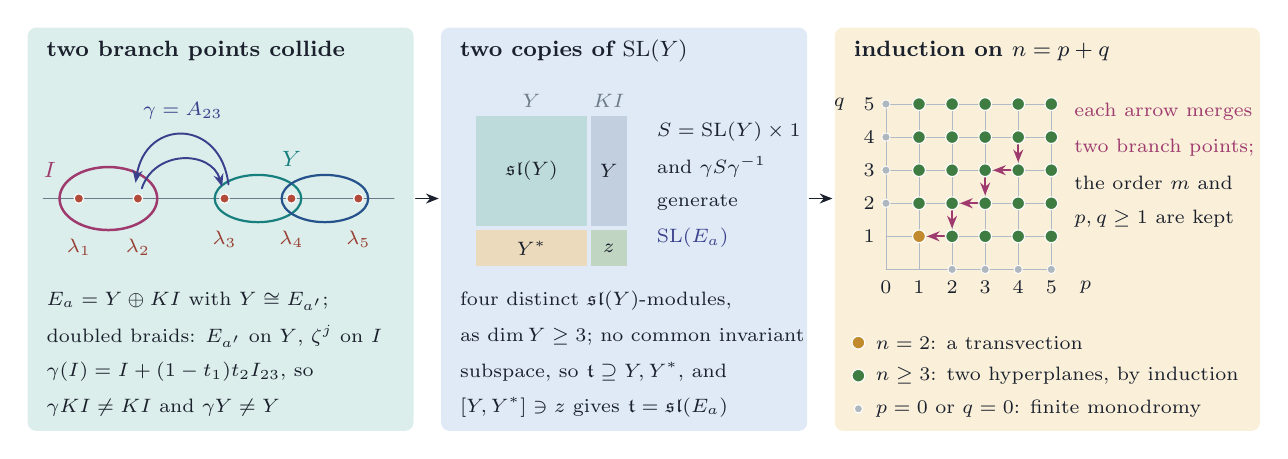
\begin{tikzpicture}[x=1cm,y=1cm,line join=round,line cap=round,
  font=\small,text=PInk,lbl/.style={inner sep=1pt}]
  \path[fill=WTeal,draw=none,rounded corners=3.0pt] (0.0500,-0.5000) rectangle (4.9500,4.6200);
  \path[fill=WBlue,draw=none,rounded corners=3.0pt] (5.3000,-0.5000) rectangle (9.9500,4.6200);
  \path[fill=PTeal!28!white,draw=none] (5.7500,2.1000) rectangle (7.1500,3.5000);
  \path[fill=PBlue!28!white,draw=none] (7.2000,2.1000) rectangle (7.6600,3.5000);
  \path[fill=POchre!32!white,draw=none] (5.7500,1.5900) rectangle (7.1500,2.0500);
  \path[fill=PGrass!32!white,draw=none] (7.2000,1.5900) rectangle (7.6600,2.0500);
  \path[fill=WOchre,draw=none,rounded corners=3.0pt] (10.3000,-0.5000) rectangle (15.7000,4.6200);
  \draw[PSlate,line width=0.6pt] (0.2500,2.4500) -- (4.7000,2.4500);
  \draw[PMag,line width=0.9pt] (1.0750,2.4500) ellipse (0.6200cm and 0.4000cm);
  \draw[PTeal,line width=0.8pt] (2.9750,2.4500) ellipse (0.5500cm and 0.3000cm);
  \draw[PBlue,line width=0.8pt] (3.8250,2.4500) ellipse (0.5500cm and 0.3000cm);
  \path[fill=PClay,draw=white,line width=0.40pt] (0.7000,2.4500) circle (1.70pt);
  \path[fill=PClay,draw=white,line width=0.40pt] (1.4500,2.4500) circle (1.70pt);
  \path[fill=PClay,draw=white,line width=0.40pt] (2.5500,2.4500) circle (1.70pt);
  \path[fill=PClay,draw=white,line width=0.40pt] (3.4000,2.4500) circle (1.70pt);
  \path[fill=PClay,draw=white,line width=0.40pt] (4.2500,2.4500) circle (1.70pt);
  \draw[PIndigo,line width=0.7pt,-{Stealth[length=4.6pt,width=3.6pt]}] (1.5000,2.5800) .. controls (1.6600,3.0700) and (2.3800,3.0700) .. (2.5200,2.6000);
  \draw[PIndigo,line width=0.7pt,-{Stealth[length=4.6pt,width=3.6pt]}] (2.6000,2.6300) .. controls (2.5000,3.4700) and (1.5500,3.4700) .. (1.4200,2.6500);
  \draw[PRule,line width=0.3pt] (10.9500,1.5500) -- (10.9500,3.6500);
  \draw[PRule,line width=0.3pt] (10.9500,1.5500) -- (13.0500,1.5500);
  \draw[PRule,line width=0.3pt] (11.3700,1.5500) -- (11.3700,3.6500);
  \draw[PRule,line width=0.3pt] (10.9500,1.9700) -- (13.0500,1.9700);
  \draw[PRule,line width=0.3pt] (11.7900,1.5500) -- (11.7900,3.6500);
  \draw[PRule,line width=0.3pt] (10.9500,2.3900) -- (13.0500,2.3900);
  \draw[PRule,line width=0.3pt] (12.2100,1.5500) -- (12.2100,3.6500);
  \draw[PRule,line width=0.3pt] (10.9500,2.8100) -- (13.0500,2.8100);
  \draw[PRule,line width=0.3pt] (12.6300,1.5500) -- (12.6300,3.6500);
  \draw[PRule,line width=0.3pt] (10.9500,3.2300) -- (13.0500,3.2300);
  \draw[PRule,line width=0.3pt] (13.0500,1.5500) -- (13.0500,3.6500);
  \draw[PRule,line width=0.3pt] (10.9500,3.6500) -- (13.0500,3.6500);
  \path[fill=PSlate!55,draw=white,line width=0.30pt] (10.9500,2.3900) circle (1.50pt);
  \path[fill=PSlate!55,draw=white,line width=0.30pt] (10.9500,2.8100) circle (1.50pt);
  \path[fill=PSlate!55,draw=white,line width=0.30pt] (10.9500,3.2300) circle (1.50pt);
  \path[fill=PSlate!55,draw=white,line width=0.30pt] (10.9500,3.6500) circle (1.50pt);
  \path[fill=POchre,draw=white,line width=0.40pt] (11.3700,1.9700) circle (2.30pt);
  \path[fill=PGrass,draw=white,line width=0.40pt] (11.3700,2.3900) circle (2.30pt);
  \path[fill=PGrass,draw=white,line width=0.40pt] (11.3700,2.8100) circle (2.30pt);
  \path[fill=PGrass,draw=white,line width=0.40pt] (11.3700,3.2300) circle (2.30pt);
  \path[fill=PGrass,draw=white,line width=0.40pt] (11.3700,3.6500) circle (2.30pt);
  \path[fill=PSlate!55,draw=white,line width=0.30pt] (11.7900,1.5500) circle (1.50pt);
  \path[fill=PGrass,draw=white,line width=0.40pt] (11.7900,1.9700) circle (2.30pt);
  \path[fill=PGrass,draw=white,line width=0.40pt] (11.7900,2.3900) circle (2.30pt);
  \path[fill=PGrass,draw=white,line width=0.40pt] (11.7900,2.8100) circle (2.30pt);
  \path[fill=PGrass,draw=white,line width=0.40pt] (11.7900,3.2300) circle (2.30pt);
  \path[fill=PGrass,draw=white,line width=0.40pt] (11.7900,3.6500) circle (2.30pt);
  \path[fill=PSlate!55,draw=white,line width=0.30pt] (12.2100,1.5500) circle (1.50pt);
  \path[fill=PGrass,draw=white,line width=0.40pt] (12.2100,1.9700) circle (2.30pt);
  \path[fill=PGrass,draw=white,line width=0.40pt] (12.2100,2.3900) circle (2.30pt);
  \path[fill=PGrass,draw=white,line width=0.40pt] (12.2100,2.8100) circle (2.30pt);
  \path[fill=PGrass,draw=white,line width=0.40pt] (12.2100,3.2300) circle (2.30pt);
  \path[fill=PGrass,draw=white,line width=0.40pt] (12.2100,3.6500) circle (2.30pt);
  \path[fill=PSlate!55,draw=white,line width=0.30pt] (12.6300,1.5500) circle (1.50pt);
  \path[fill=PGrass,draw=white,line width=0.40pt] (12.6300,1.9700) circle (2.30pt);
  \path[fill=PGrass,draw=white,line width=0.40pt] (12.6300,2.3900) circle (2.30pt);
  \path[fill=PGrass,draw=white,line width=0.40pt] (12.6300,2.8100) circle (2.30pt);
  \path[fill=PGrass,draw=white,line width=0.40pt] (12.6300,3.2300) circle (2.30pt);
  \path[fill=PGrass,draw=white,line width=0.40pt] (12.6300,3.6500) circle (2.30pt);
  \path[fill=PSlate!55,draw=white,line width=0.30pt] (13.0500,1.5500) circle (1.50pt);
  \path[fill=PGrass,draw=white,line width=0.40pt] (13.0500,1.9700) circle (2.30pt);
  \path[fill=PGrass,draw=white,line width=0.40pt] (13.0500,2.3900) circle (2.30pt);
  \path[fill=PGrass,draw=white,line width=0.40pt] (13.0500,2.8100) circle (2.30pt);
  \path[fill=PGrass,draw=white,line width=0.40pt] (13.0500,3.2300) circle (2.30pt);
  \path[fill=PGrass,draw=white,line width=0.40pt] (13.0500,3.6500) circle (2.30pt);
  \draw[PMag,line width=0.7pt,-{Stealth[length=4.6pt,width=3.6pt]}] (12.6300,3.1300) -- (12.6300,2.9100);
  \draw[PMag,line width=0.7pt,-{Stealth[length=4.6pt,width=3.6pt]}] (12.5300,2.8100) -- (12.3100,2.8100);
  \draw[PMag,line width=0.7pt,-{Stealth[length=4.6pt,width=3.6pt]}] (12.2100,2.7100) -- (12.2100,2.4900);
  \draw[PMag,line width=0.7pt,-{Stealth[length=4.6pt,width=3.6pt]}] (12.1100,2.3900) -- (11.8900,2.3900);
  \draw[PMag,line width=0.7pt,-{Stealth[length=4.6pt,width=3.6pt]}] (11.7900,2.2900) -- (11.7900,2.0700);
  \draw[PMag,line width=0.7pt,-{Stealth[length=4.6pt,width=3.6pt]}] (11.6900,1.9700) -- (11.4700,1.9700);
  \path[fill=POchre,draw=white,line width=0.40pt] (10.6000,0.6200) circle (2.30pt);
  \path[fill=PGrass,draw=white,line width=0.40pt] (10.6000,0.2000) circle (2.30pt);
  \path[fill=PSlate!55,draw=white,line width=0.40pt] (10.6000,-0.2200) circle (1.50pt);
  \draw[PInk,line width=0.6pt,-{Stealth[length=4.6pt,width=3.6pt]}] (4.9800,2.4500) -- (5.2700,2.4500);
  \draw[PInk,line width=0.6pt,-{Stealth[length=4.6pt,width=3.6pt]}] (9.9800,2.4500) -- (10.2700,2.4500);
  \node[lbl,anchor=west,text=PInk,font=\footnotesize] at (0.2500,4.3200) {\textbf{two branch points collide}};
  \node[lbl,anchor=north,text=PClay!85!black,font=\scriptsize] at (0.7000,1.9800) {$\lambda_{1}$};
  \node[lbl,anchor=north,text=PClay!85!black,font=\scriptsize] at (1.4500,1.9800) {$\lambda_{2}$};
  \node[lbl,anchor=north,text=PClay!85!black,font=\scriptsize] at (2.5500,2.0800) {$\lambda_{3}$};
  \node[lbl,anchor=north,text=PClay!85!black,font=\scriptsize] at (3.4000,2.0800) {$\lambda_{4}$};
  \node[lbl,anchor=north,text=PClay!85!black,font=\scriptsize] at (4.2500,2.0800) {$\lambda_{5}$};
  \node[lbl,anchor=east,text=PMag,font=\footnotesize] at (0.4500,2.8082) {$I$};
  \node[lbl,anchor=south,text=PTeal,font=\footnotesize] at (3.4000,2.8100) {$Y$};
  \node[lbl,anchor=south,text=PIndigo,font=\scriptsize] at (2.0200,3.4100) {$\gamma=A_{23}$};
  \node[lbl,anchor=west,text=PInk,font=\scriptsize] at (0.2500,1.1500) {$E_{a}=Y\oplus KI$ with $Y\cong E_{a'}$;};
  \node[lbl,anchor=west,text=PInk,font=\scriptsize] at (0.2500,0.7000) {doubled braids: $E_{a'}$ on $Y$, $\zeta^{j}$ on $I$};
  \node[lbl,anchor=west,text=PInk,font=\scriptsize] at (0.2500,0.2500) {$\gamma(I)=I+(1-t_{1})t_{2}I_{23}$, so};
  \node[lbl,anchor=west,text=PInk,font=\scriptsize] at (0.2500,-0.2000) {$\gamma KI\ne KI$ and $\gamma Y\ne Y$};
  \node[lbl,anchor=west,text=PInk,font=\footnotesize] at (5.5000,4.3200) {\textbf{two copies of $\mathrm{SL}(Y)$}};
  \node[lbl,text=PInk,font=\scriptsize] at (6.4500,2.8000) {$\mathfrak{sl}(Y)$};
  \node[lbl,text=PInk,font=\scriptsize] at (7.4300,2.8000) {$Y$};
  \node[lbl,text=PInk,font=\scriptsize] at (6.4500,1.8200) {$Y^{*}$};
  \node[lbl,text=PInk,font=\scriptsize] at (7.4300,1.8200) {$z$};
  \node[lbl,anchor=south,text=PSlate,font=\scriptsize] at (6.4500,3.5600) {$Y$};
  \node[lbl,anchor=south,text=PSlate,font=\scriptsize] at (7.4300,3.5600) {$KI$};
  \node[lbl,anchor=west,text=PInk,font=\scriptsize] at (8.0000,3.3000) {$S=\mathrm{SL}(Y)\times1$};
  \node[lbl,anchor=west,text=PInk,font=\scriptsize] at (8.0000,2.8500) {and $\gamma S\gamma^{-1}$};
  \node[lbl,anchor=west,text=PInk,font=\scriptsize] at (8.0000,2.4000) {generate};
  \node[lbl,anchor=west,text=PIndigo,font=\scriptsize] at (8.0000,1.9500) {$\mathrm{SL}(E_{a})$};
  \node[lbl,anchor=west,text=PInk,font=\scriptsize] at (5.5000,1.1500) {four distinct $\mathfrak{sl}(Y)$-modules,};
  \node[lbl,anchor=west,text=PInk,font=\scriptsize] at (5.5000,0.7000) {as $\dim Y\ge3$; no common invariant};
  \node[lbl,anchor=west,text=PInk,font=\scriptsize] at (5.5000,0.2500) {subspace, so $\mathfrak{t}\supseteq Y,Y^{*}$, and};
  \node[lbl,anchor=west,text=PInk,font=\scriptsize] at (5.5000,-0.2000) {$[Y,Y^{*}]\ni z$ gives $\mathfrak{t}=\mathfrak{sl}(E_{a})$};
  \node[lbl,anchor=west,text=PInk,font=\footnotesize] at (10.5000,4.3200) {\textbf{induction on $n=p+q$}};
  \node[lbl,anchor=north,text=PInk,font=\scriptsize] at (10.9500,1.4500) {$0$};
  \node[lbl,anchor=north,text=PInk,font=\scriptsize] at (11.3700,1.4500) {$1$};
  \node[lbl,anchor=east,text=PInk,font=\scriptsize] at (10.8500,1.9700) {$1$};
  \node[lbl,anchor=north,text=PInk,font=\scriptsize] at (11.7900,1.4500) {$2$};
  \node[lbl,anchor=east,text=PInk,font=\scriptsize] at (10.8500,2.3900) {$2$};
  \node[lbl,anchor=north,text=PInk,font=\scriptsize] at (12.2100,1.4500) {$3$};
  \node[lbl,anchor=east,text=PInk,font=\scriptsize] at (10.8500,2.8100) {$3$};
  \node[lbl,anchor=north,text=PInk,font=\scriptsize] at (12.6300,1.4500) {$4$};
  \node[lbl,anchor=east,text=PInk,font=\scriptsize] at (10.8500,3.2300) {$4$};
  \node[lbl,anchor=north,text=PInk,font=\scriptsize] at (13.0500,1.4500) {$5$};
  \node[lbl,anchor=east,text=PInk,font=\scriptsize] at (10.8500,3.6500) {$5$};
  \node[lbl,anchor=west,text=PInk,font=\scriptsize] at (13.3700,1.3300) {$p$};
  \node[lbl,anchor=east,text=PInk,font=\scriptsize] at (10.4700,3.6500) {$q$};
  \node[lbl,anchor=west,text=PMag,font=\scriptsize] at (13.3000,3.5500) {each arrow merges};
  \node[lbl,anchor=west,text=PMag,font=\scriptsize] at (13.3000,3.1000) {two branch points;};
  \node[lbl,anchor=west,text=PInk,font=\scriptsize] at (13.3000,2.6500) {the order $m$ and};
  \node[lbl,anchor=west,text=PInk,font=\scriptsize] at (13.3000,2.2000) {$p,q\ge1$ are kept};
  \node[lbl,anchor=west,text=PInk,font=\scriptsize] at (10.7800,0.6200) {$n=2$: a transvection};
  \node[lbl,anchor=west,text=PInk,font=\scriptsize] at (10.7800,0.2000) {$n\ge3$: two hyperplanes, by induction};
  \node[lbl,anchor=west,text=PInk,font=\scriptsize] at (10.7800,-0.2200) {$p=0$ or $q=0$: finite monodromy};
\end{tikzpicture}
\end{document}
